\chapter{Processo de engenharia de requisitos}

  Texto Texto Texto Texto Texto Texto Texto Texto Texto Texto Texto Texto Texto Texto
  Texto Texto Texto Texto Texto Texto Texto Texto Texto Texto Texto Texto Texto Texto
  Texto Texto Texto Texto Texto Texto Texto Texto Texto Texto Texto Texto Texto Texto
  Texto Texto Texto Texto Texto Texto Texto Texto Texto Texto Texto Texto Texto Texto

\section{Maturidade}
  \subsection{CMMI (Capability Maturity Model - Integration)}

  O CMMI é um modelo de maturidade internacional, geralmente utilizado por empresas
  globalizadas que necessitam de certificação para serem reconhecidos internacionalmente.
  Surgiu como integração e evolução dos modelos SW-CMM (Capability Maturity Model for Software),
  SECM EIA 731 (System Engineering Capability Model) e  e IPD-CMM
  (Integrated Product Development CMM) \cite{mct2006}.
  O CMMI possui 5 níveis de maturidade, enumerdos do 1 ao 5 e cada nível corresponde
  à capacidade da organização de desenvolvimento do produto, sendo o nível 1 o mais
  baixo nível de maturidade e o nível 5 o mais alto e contínuo.

  \begin{figure}[!ht]
    \centering
    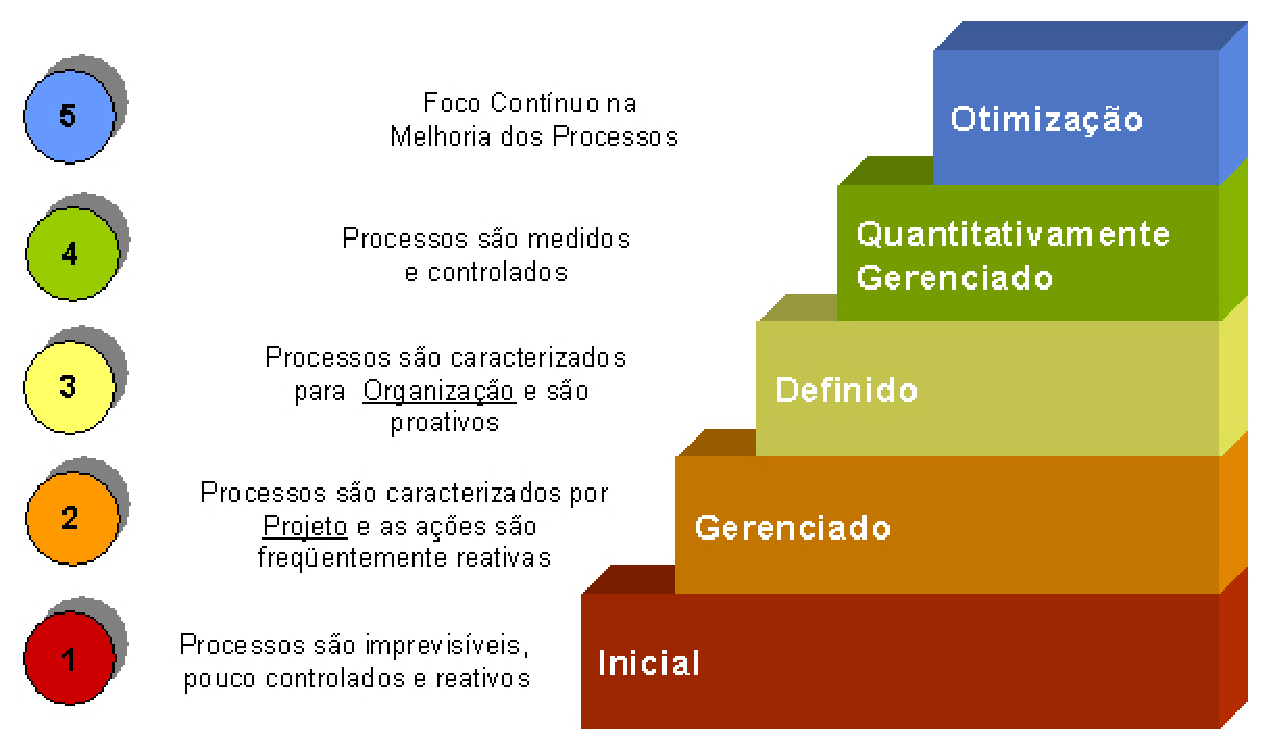
\includegraphics[width=15cm, keepaspectratio=true]{figuras/maturidade/niveis-cmmi.eps}
    \caption{Os cinco níveis de maturidade do modelo CMMI e suas respectivas descrições.}
  \end{figure}

    \subsubsection{Vantagens}

    Como já dito na descrição na Subseção 1.1, o CMMI é um modelo de melhoria
    de processos reconhecido internacionalmente, fazendo com que a organização
    certificada por ele tenha a vantagem de ser reconhecida em qualquer lugar
    do mundo por causa da aplicação do CMMI.
    Com o CMMI, a organização vai se otimizando cada vez mais e o controle do
    processo fica cada vez mais definido, sendo assim, a organização continuamente
    vai identificando o que realmente tem valor de acordo com sua maturidade.

    \subsubsection{Desvantagens}

    O CMMI tem um alto custo, por isso geralmente quem tem a certificação são
    grandes organizações globalizadas que possuem recursos para sustentar a
    avaliação e se torna vantajoso para seu reconhecimento internacional. O
    tempo para amadurecimento do processo pode levar de 4 a 8 anos, sendo assim
    definido um modelo moroso e caro. Segundo Franciscani, algumas organizações
    tratam o CMMi como um processo e não como modelo, fazendo com que eles tenham
    a percepção de que nem tudo que está no CMMI seja mesmo necesário
    \cite{francis2012}.


  \subsection{MPS.BR}

  O modelo MPS.BR foi desenvolvido pela Softex com o objetivo de atingir
  certificações de pequenas e médias empresas, bem como possibilitar que
  as empresas possam ter acesso mais facilitado para a certificação.
  O modelo MPS.BR se adequa ao mercado brasileiro de software e deriva do CMMI.
  Enquanto o CMMI possui cinco níveis de maturidade enumeradas do 1 ao 5, o
  MPS.BR possui sete níveis classificados, de forma piramidal,  pelas letras
  do A ao G, sendo o nível A o mais alto e contínuo nível de maturidade e o G
  o mais baixo. A Figura 2 contém a representação dos níveis de maturidade do
  MPS.BR.

  \begin{figure}[!ht]
    \centering
    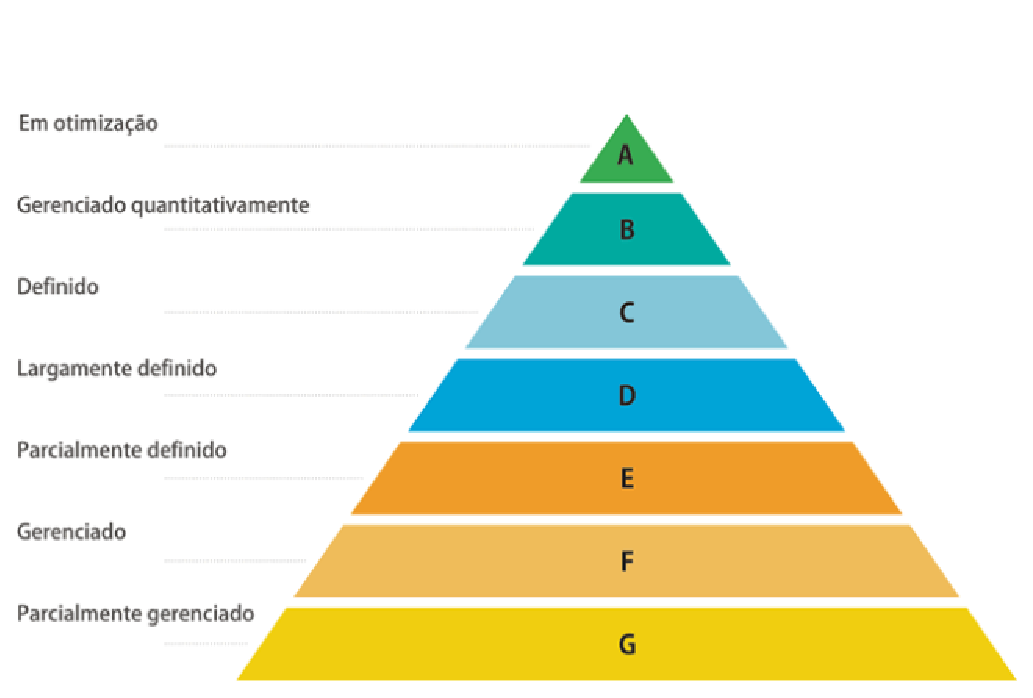
\includegraphics[width=15cm, keepaspectratio=true]{figuras/maturidade/niveis-mpsbr.eps}
    \caption{Os sete níveis de maturidade do modelo MPS.BR e suas respectivas descrições. Os
              níveis de maturidade do MPS.BR não são enumerados, mas representados por letras
              que vão do A ao G.}
  \end{figure}

    \subsubsection{Vantagens}

    Além do MPS.BR ser mais acessível e estar mais adequado ao contexto de
    organizações brasileiras, segundo Franciscani, existem outras vantagens
    como:

    \begin{itemize}
      \item{Compatibilidade com CMMI, podendo ser aproveitado para uma futura
            certificação nesse modelo.}
      \item{Dois números de nível a mais do que do CMMI, o que pode facilitar a
            implantação em pequenas e médias organizações.}
      \item{Obrigatoriedade do certificado em licitações.}
      \item{Integração Universidade-Empresa.}
    \end{itemize}

    \subsubsection{Desvantagens}

    O MPS.BR não possibilita as empresas serem competitivas internacionalmente,
    por ser um modelo que se adequa apenas para certificação nacional. Isso pode
    ser uma desvantagem muito grande para organizações que pretendem
    globalizar-se \cite{francis2012}.

  \subsection{Seleção do Modelo}

    A Cráton é uma empresa júnior com apenas 15 membros formada por estudantes no qual
    não visam lucro para si mesmos, pois todo o dinheiro obtido deve ser investido
    na própria empresa como consta na lei número 13.267 de 2016 que regulamenta as empresas
    juniores e as define com fim educacional e não lucrativo. Neste contexto, o CMMI seria
    impraticável devido ao alto custo e a limitação de crescimento de uma empresa júnior que é
    completamente dependente das universidades e não seria globalizada, não precisando do CMMI.

    O grupo possui quatro integrantes, o que se encaixa no contexto do MPS.BR que se direciona
    principalmente para organizações menores, fazendo-se ser mais acessível para poder desenvolver
    o modelo dentro do contexto do cliente.

    O cliente, sendo uma empresa júnior integrada com a Universidade de Brasília, poderia se
    beneficiar dos processos do MPS.BR, já que é um modelo que possui integração universidade-empresa.
    Dessa forma, o modelo seria aplicado diretamente no meio acadêmico.

    Por esses motivos apontados, o modelo MPS.BR foi selecionado para a engenharia de requisitos da
    solução do problema da Cráton.

  \subsection{Processos Selecionados}

  Para o contexto da disciplina, serão implementados dois processos que tratam de
  requisitos, sendo o processo de Gerência de Requisitos que se encontra no nível
  G do MPS.BR e o Desenvolvimento de Requisitos que é um processo do nível D. Nos
  subtópicos seguintes, 1.4.1 e 1.4.2, estará o propósito e os resultados esperados
  de cada processo referenciado diretamente do Guia Geral do MPS.BR \cite{softexmps}.

    \subsubsection{Gerência de Requisitos - GRE}
      \begin{description}
        \item[Propósito]

      O propósito do processo Gerência de Requisitos é gerenciar os requisitos do
      produto e dos componentes do produto do projeto e identificar inconsistências
      entre os requisitos, os planos do projeto e os produtos de trabalho do projeto.

      \item [Resultados Esperados]

      \begin{itemize}
        \item GRE 1. O entendimento dos requisitos é obtido junto aos fornecedores de requisitos;
        \item GRE 2. Os requisitos são avaliados com base em critérios objetivos e um comprometimento
              da equipe técnica com estes requisitos é obtido;
        \item GRE 3. A rastreabilidade bidirecional entre os requisitos e os produtos de trabalho
              é estabelecida e mantida;
        \item GRE 4. Revisões em planos e produtos de trabalho do projeto são realizadas;
              visando identificar e corrigir inconsistências em relação aos requisitos;
        \item GRE 5. Mudanças nos requisitos são gerenciadas ao longo do projeto.
      \end{itemize}
    \end{description}

    \subsubsection{Desenvolvimento de Requisitos - DRE}
    \begin{description}
      \item [Propósito] \

       O propósito do processo Desenvolvimento de Requisitos é definir os requisitos
       do cliente, do produto e dos componentes do produto.

      \item [Resultados Esperados]\

      \begin{itemize}
        \item DRE 1. As necessidades, expectativas e restrições do cliente, tanto do produto
              quanto de suas interfaces, são identificadas;
        \item DRE 2. Um conjunto definido de requisitos do cliente é especificado e priorizado
              a partir das necessidades, expectativas e restrições identificadas;
        \item DRE 3. Um conjunto de requisitos funcionais e não-funcionais, do produto e dos componentes
                    do produto que descrevem a solução do problema a ser resolvido, é definido e mantido
                    a partir dos requisitos do cliente;
        \item DRE 4. Os requisitos funcionais e não-funcionais de cada componente do produto são
              refinados, elaborados e alocados;
        \item DRE 5. Interfaces internas e externas do produto e de cada componente do produto são
              definidas;
        \item DRE 6. Conceitos operacionais e cenários são desenvolvidos;
        \item DRE 7. Os requisitos são analisados, usando critérios definidos, para balancear
              as necessidades dos interessados com as restrições existentes;
        \item DRE 8. Os requisitos são validados.
      \end{itemize}
    \end{description}
